% https://de.overleaf.com/latex/templates/a-quick-guide-to-latex/fghqpfgnxggz

\documentclass[10pt]{article}
% ========== Packages ==========
\usepackage[a4paper,
  left=10mm,
  right=10mm,
  top=10mm,
  bottom=17mm
]{geometry}

% \usepackage[ngerman]{babel} %Ändert die Sprache
\usepackage[T1]{fontenc} %Wichtig für ä ö ü
\usepackage{amssymb,amsmath,amsthm,amsfonts}
\usepackage{graphicx}
\usepackage{fancyhdr}
\usepackage[utf8]{inputenc}
\usepackage{multicol,multirow}
\usepackage{longtable} %Für lange Tabellen
\usepackage{arydshln} %Für gestrichelte Linien in Tabellen
\usepackage{tabularx}
\usepackage{pdfpages} %Zum einfügen von PDF's
\usepackage{hyperref} %Für hyperlinks
\hypersetup{bookmarks=true}
\usepackage{parskip}
\usepackage{caption} %Für die Beschriftung von Bilder
\captionsetup{justification=centering}
\captionsetup{font=it}
\setlength{\parindent}{0pt}
\usepackage{subcaption} %Für die Beschriftung unterteilter Bilder
\usepackage{float}
\floatstyle{plaintop}
\restylefloat{table}
\usepackage{siunitx}%Für einheiten im Symbolverzeichnis
% \usepackage[symbols,nogroupskip,sort=none]{glossaries-extra}%Für Symbolverzeichnis
% % \input{symbolverzeichnis}
\usepackage{lipsum}%Für pseudo text



\makeatletter %Für römische Zahlen
\newcommand*{\rom}[1]{\expandafter\@slowromancap\romannumeral #1@}

%Für die dicken Linien in Tabellen
\def\thickhline{%
  \noalign{\ifnum0=`}\fi\hrule \@height \thickarrayrulewidth \futurelet
   \reserved@a\@xthickhline}
\def\@xthickhline{\ifx\reserved@a\thickhline
               \vskip\doublerulesep
               \vskip-\thickarrayrulewidth
               \fi
      \ifnum0=`{\fi}}
\makeatother
\newlength{\thickarrayrulewidth}
\setlength{\thickarrayrulewidth}{2\arrayrulewidth}

%Sorgt dafür, dass nicht immer alles auf die ganze Seite verteilt wird.
\raggedbottom

% ========== Header and Footer ==========
\pagestyle{fancy}
\fancyhf{}
% \fancyhead[RE,LO]{Seite \thepage}
% \fancyhead[LE,RO]{\nouppercase{\leftmark}}
\fancyfoot[RE,LO]{Page \thepage}
\renewcommand{\headrulewidth}{0pt}
\renewcommand{\footrulewidth}{.5pt}

%Eigens erstellte Variablen
\newcommand{\plotWidth}{0.7}
\newcommand{\garphWidth}{0.7}
\newcommand{\linienAbstand}{2ex}
\newcommand{\linienDicke}{0.5pt}
\newcommand{\linienDickeDick}{1.5pt}


% \usepackage{calc}
% \usepackage{ifthen}
% \ifthenelse{\lengthtest { \paperwidth = 11in}}
%     { \geometry{top=.5in,left=.5in,right=.5in,bottom=.5in} }
% 	{\ifthenelse{ \lengthtest{ \paperwidth = 297mm}}
% 		{\geometry{top=1cm,left=1cm,right=1cm,bottom=1cm} }
% 		{\geometry{top=1cm,left=1cm,right=1cm,bottom=1cm} }
% 	}
% \pagestyle{empty}
\makeatletter
\renewcommand{\section}{\@startsection{section}{1}{0mm}%
                                {-1ex plus -.5ex minus -.2ex}%
                                {0.5ex plus .2ex}%x
                                {\normalfont\large\bfseries}}
\renewcommand{\subsection}{\@startsection{subsection}{2}{0mm}%
                                {-1explus -.5ex minus -.2ex}%
                                {0.5ex plus .2ex}%
                                {\normalfont\normalsize\bfseries}}
\renewcommand{\subsubsection}{\@startsection{subsubsection}{3}{0mm}%
                                {-1ex plus -.5ex minus -.2ex}%
                                {1ex plus .2ex}%
                                {\normalfont\small\bfseries}}
\makeatother
\setcounter{secnumdepth}{0}
\setlength{\parindent}{0pt}
\setlength{\parskip}{0pt plus 0.5ex}
% -----------------------------------------------------------------------


\begin{document}
\footnotesize

\begin{center}
     \Large{\textbf{Ordinary Differential Equations and Dynamical Systems}} \\
\end{center}
\begin{multicols}{2}
\setlength{\premulticols}{1pt}
\setlength{\postmulticols}{1pt}
\setlength{\multicolsep}{1pt}
\setlength{\columnsep}{2pt}
\raggedbottom

% Part I
\part{Modeling}
\section{Fundamentals}
\noindent\rule[\linienAbstand]{\linewidth}{\linienDickeDick}
Formally, an ordinary differential equation is an equation, in which a function and its derivates and the independent variable appear.\\

An (implicit) \emph{ordinary differential equation} of order n is an equation of the form
\begin{equation}
  F(x, y, y', y'', ..., y^{(n)}) = 0.
\end{equation}
An example of an explicit ODE of order $n$ is of the form
\begin{equation}
  y^{n} = G(x, y, y', y'', ..., y^{n-1}).
\end{equation}

\section{Classification}
\noindent\rule[\linienAbstand]{\linewidth}{\linienDickeDick}

Differential equations can be classified according to various criteria. Besides the order of an ODE we are also interested in whether an ODE is linear, homogeneous, has constant coefficient, is separable or autonomous.\\

\textbf{Linearity}\\
An \emph{n-th} order ODE is \emph{linear}, if it is of the form:
\begin{equation}
  a_n(x) \cdot y^{(n)} + ... + a_1(x) \cdot y' + a_0(x) \cdot y = g(x)
\end{equation}
where $a_n(x), ..., a_1(x), a_0(x)$ are $g(x)$ fixed functions. Or in other words: A differential equation is linear if the dependant variable and all of its derivatives appear in a linear fashion (i.e., they are not multiplied together or squared for example or they are not part of transcendental functions such as sins, cosines, exponentials, etc.)\\\\

\textbf{Homogenity}\\
A lienar ODE is \emph{homogeneous}, if $g(x) = 0$ for all $x$; otherwise the ODE is \emph{inhomogeneous}, and $g(x)$ is the \emph{inhomogeneity} or \emph{source} term.\\

\textbf{Constant coefficient}\\
A linear ODE has \emph{constant coefficients}, if it is of the form
\begin{equation}
  a_n \cdot y^{(n)} + ... + a_1 \cdot y'+ a_0 \cdot y = g(x),
\end{equation}
with $a_n \neq 0$ (the source term $g(x)$ does not have to be constant).\\

\textbf{Separability}\\
The ODE is \emph{separable}, if $F(x, y)$ can be written as a product of a $x$- and $y$-dependent term, i.e. if the ODE is of the form
\begin{equation}
  y' = g(x) \cdot h(y)
\end{equation}

\textbf{Autonomity}\\
The ODE (1.28) is \emph{autonomous}, if $F(x, y)$ only depends on $y$, i.e. if the ODE is of the form
\begin{equation}
  y' = h(y)
\end{equation}
Every autonomous ODE is separable with $g(x) = 1$.\\

\textbf{Examples}\\
\begin{tabular}{ll}
  $y' = f(x)$ & Inhomogeneous linear ODE for $y(x)$ with\\
  & source term $f(x)$\\
  $m \cdot \dot{v} = m \cdot g - k \cdot v^2$ & Nonlinear ODE for $v(t)$\\
  $l \cdot \ddot{\Phi} + g \cdot sin(\Phi) = 0$ & Nonlinear ODE for $\Phi(t)$\\
  $l \cdot \ddot{\Phi} + g \cdot \phi$ & Homogeneous linear ODE for $\Phi(t)$\\
  $l \cdot \ddot{\Phi} + g \cdot \phi = sin(\omega t)$ & Inhomogeneous linear ODE for $\Phi(t)$ with\\
  & source term $sin(\omega t)$\\
  $i''+ \frac{R}{L}i' + \frac{1}{LC}i = 0$ & Homogeneous linear ODE for $i(t)$
\end{tabular}

\section{Systems of differential equations}
\noindent\rule[\linienAbstand]{\linewidth}{\linienDickeDick}
If several systems are coupled with each other and mutually influence each other, one often obtains a system of ODE’s.\\
A \emph{system of differential equations} of first order is a system
\begin{equation}
  \begin{matrix}
    y'_1 & = & f_1(x, y_1,...,y_n)\\
    \vdots & & \vdots \;\;\;\;\; \; \; \; \; \; \; \; \; \; \; \; \; \; \\
    y'_n & = & f_n(x, y_1,...,y_n)
\end{matrix}
\end{equation}
of ODE’s for unknown functions $y_1(x), ... , y_n(x)$.\\
Using the vectorial notation
\begin{equation}
  \mathbf{y}' = \mathbf{f}(x, \mathbf{y})
\end{equation}

An ODE of \emph{n}-th order is equivalent to a system of first-order ODE's.
\begin{equation}
  \begin{matrix}
    y_1' & = & y_2\\
    y_2' & = & y_3\\
    \vdots  &  & \vdots \\
    y_n' & = & f(x, y_1, ..., y_n)
  \end{matrix}
\end{equation}

\textbf{Example: 2nd-order ODE to system of first-order ODE's}\\
We want to rewrite the following 2$nd$ order ODE into a system of first-order ODE's.
\begin{equation}
  \ddot{x}(t) + 2\delta\dot{x}(t) + \omega_0^2x(t) = f(t)
\end{equation}
If we introduce the vector-valued function
\begin{equation}
  \textup{y} = \begin{pmatrix} y_1 \\ y_2 \end{pmatrix} =
                \begin{pmatrix} x \\ \dot{x} \end{pmatrix} \;\;\;\;  \Rightarrow \;\;\;\;
                \dot{\textup{y}} =
                \begin{pmatrix} \dot{y_1} \\ \dot{y_2} \end{pmatrix} =
                \begin{pmatrix} \dot{x} \\ \ddot{x} \end{pmatrix}
\end{equation}
rewriting:
\begin{equation}
  \begin{split}
      \dot{\textup{y}} =& \begin{pmatrix} \dot{x} \\ \ddot{x} \end{pmatrix} =
                          \begin{pmatrix} \dot{x} \\ -2\delta\dot{x}(t) - \omega_0^2x(t) + f(t) \end{pmatrix}\\
      \dot{\textup{y}} =& \begin{pmatrix} \dot{x} \\ \ddot{x} \end{pmatrix} =
                          \begin{pmatrix} 0 & 1 \\ -\omega_0^2 & -2\delta \end{pmatrix}
                          \begin{pmatrix} x\\ \dot{x} \end{pmatrix} +
                          \begin{pmatrix} 0 \\ f(t) \end{pmatrix}\\
      \dot{\textup{y}} =& \textup{A}\textbf{y} + \mathbf{b}
  \end{split}
\end{equation}

\section{Slope field}
\noindent\rule[\linienAbstand]{\linewidth}{\linienDickeDick}
Slope fields are often loead to a good qualitative understanding of the situation described by the ODE under consideration.
Slope field can be understood in the following way: To each point $(x, y)$ in the region $B$ under consideration, $F(x, y)$ is a value which discribes the slope of the solution curve passing through the point $(x, y)$.\\

\textbf{Example with calculator}\\
We want to plot the slope field of the following ODE
\begin{equation}
  y' = x - y
\end{equation}
\begin{table}[H]
  \setlength{\tabcolsep}{0.2em}
  \footnotesize
  \begin{tabular}{p{\linewidth / 2 - 0.5em}@{\hskip 1em}p{\linewidth / 2 - 0.5em}}
    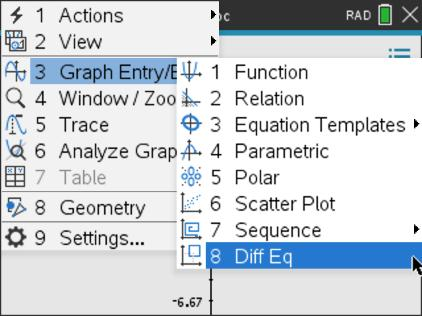
\includegraphics[width=\linewidth]{Pics/1.5.1.jpg} & 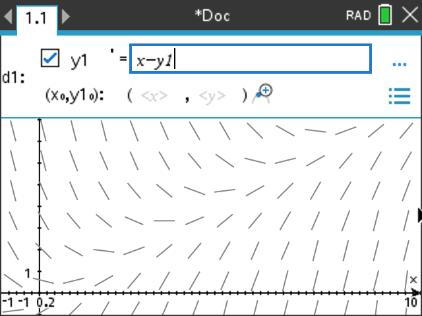
\includegraphics[width=\linewidth]{Pics/1.5.2.jpg} \\
    Select: Menu, 3: Graph Entry/Edit, 8: Diff Eq. & Write down the ODE
  \end{tabular}
\end{table}




\end{multicols}
\end{document}
